\section{Case study: slick-direct} % (fold)
\label{sec:CaseStudy}
Slick~\autocite{typesafe_slick_2015} is a popular Scala library used to query databases.
Slick is recommended by Typesafe as the functional relational mapper for their well known Play framework.
Professional Scala consultancies such as \href{http://underscore.io}{underscore.io} offer public and private training on Slick and underscore.io even recently released a book about the library\footnote{http://underscore.io/training/courses/essential-slick/}.
The hefty prices on the private training indicates that there is commercial interest in using Slick.
The fact that the book is close to 300 pages may also indicate that the library has a steep learning curve.

We chose to evaluate Directembedding by implementing a front-end for Slick for a few reasons.
Firstly, Slick is a widely used library in the industry.
Secondly, the lifted embedding API is quite elaborate and uses many advanced features of the Scala type system.
Thirdly, there exists a lot of related work on direct embedding for Slick.

In this case study, we compare in detail the lifted embedding with our implementation of the direct embedding.
Sections~\ref{sub:LiftedEmbedding} and~\ref{sub:Directembedding} cover how queries are created in the lifted embedding and direct embedding, respectively.
% In Section~\ref{sub:TypeSignatures}, we look into the differences between the type signatures in the lifted embedding and direct embedding.
% In , we consider the trade-offs that we took to implement slick-direct.
In Section~\ref{sub:Relatedwork}, we look at the related work on direct embedding with Slick.

\subsection{Lifted embedding} % (fold)
\label{sub:LiftedEmbedding}
The lifted embedding is the recommended way to query data with Slick.
The supertype of all members in the lifted embedding is the \texttt{slick.lifted.Rep[T]} trait.
Figure~\ref{fig:rep} shows the type hierarchy of \texttt{Rep[T]}.
To create a query with the lifted embedding, a Slick user must in one way or another interact with all subtypes in the hierarchy.
\begin{figure}
    \centering
    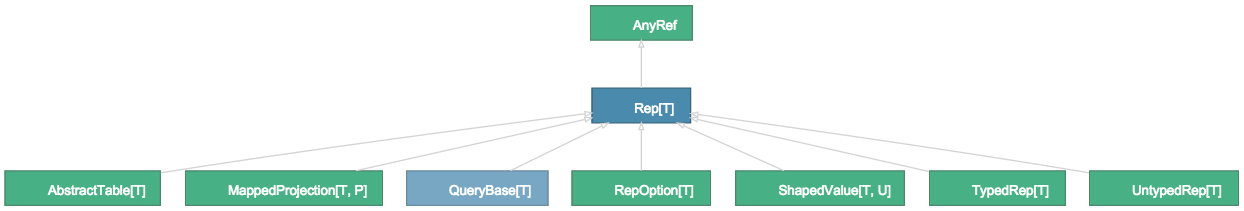
\includegraphics[width=\textwidth]{img/rep.png}
    \caption{The type hierarchy of \texttt{slick.lifted.Rep[T]} in Slick.}\label{fig:rep}
\end{figure}
The purpose of the lifted embedding API is to create an abstract syntax tree (AST) of type \texttt{slick.ast.Node}, which is then passed onto the query optimization engine of Slick.
In the next few paragraphs, we will follow an example to see how a query inside the lifted embedding is created from the point of view of a Slick users.
% The \texttt{Node} API will not be discussed until Section~\ref{sub:alternatives}.
The following example is made up of simple database of users and cars owned our users and is split into four steps.
Observe that some details such as database drivers are left out for clarity.
% Figure~\ref{fig:node} shows the type hierarchy of \texttt{Node}.
% \begin{figure}
%     \centering
%     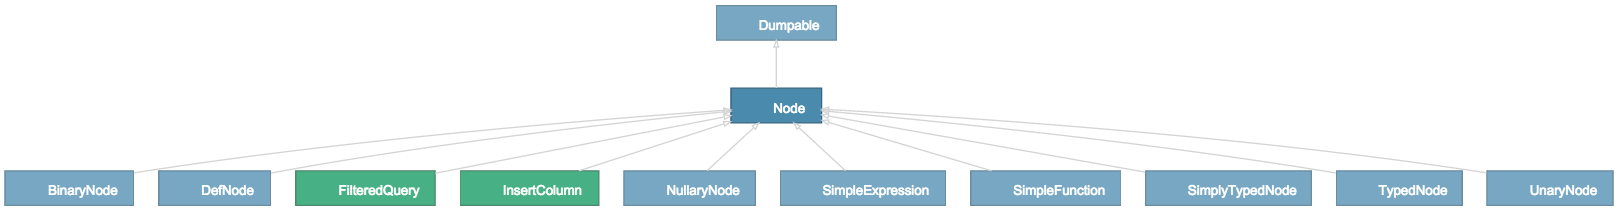
\includegraphics[width=\textwidth]{img/node.png}
%     \caption{The type hierarchy of \texttt{slick.ast.Node} in Slick.}\label{fig:node}
% \end{figure}


Listing~\ref{lst:oo} shows the definitions of our basic Scala classes: \texttt{User} and \texttt{Car}.
\lstinputlisting[label={lst:oo}, float, caption=Original case classes]{code/oo.scala}
These classes will be the values which we want to insert into and fetch from our database.

Listing~\ref{lst:table} shows our \texttt{Table[T]} definitions, where we provide necessary metadata to query on our user and car objects.
\lstinputlisting[label={lst:table}, float, caption=\texttt{Table[T]} definition, float]{code/table.scala}
Observe that the names of the members in our standard user and car objects are repeated at least four times:
\begin{inparaenum}[i)]
    \item in the case class definition,
    \item in the method names in the table definition,
    \item in the string literals to identify the column names in the database, and
    \item in the \texttt{ProvenShape} mapping in the \texttt{$\ast$} method.
\end{inparaenum}
In the case of the \texttt{ownerId} --- which has the foreign key constraint --- we must repeat the name two more times, a combined of six times.
The benefit to this table definition is that it gives great flexibility to the user.
The downside is that the table definition forces a lot of boilerplate onto users --- violates DRY --- and may be likely to introduce bugs in the code.
To alleviate this issue, Slick provides a library to generate these table definitions from a database schema.

Listing~\ref{lst:tablequery} shows how we create \texttt{TableQuery} objects, which we use to write queries.
\lstinputlisting[label=lst:tablequery, float, caption=\texttt{TableQuery[T]} definition]{code/tablequery.scala}
Queries are written with a similar syntax as with Scala collections.
Listing~\ref{lst:query} shows several examples of Slick queries and their corresponding translations to (simplified) SQL.\
\lstinputlisting[label=lst:query, float, caption=Slick queries]{code/example-queries.scala}\label{}
Take a moment to appreciate some of the benefits to writing queries like this:
Queries can be type-checked;
IDEs can provide auto-completion to the end user; and
if a user knows how to operate on Scala collections the user can write SQL.\
Once we invoke a \texttt{map} or \texttt{filter} operation on a \texttt{TableQuery[T]}, we get a value of type \texttt{Query[E, T, C]} where in our example
\begin{inparaenum}[i)]
\item \texttt{E} will be \texttt{Users} and \texttt{Cars},
\item \texttt{T} will be \texttt{User} and \texttt{Car}, and
\item \texttt{C} will typically be the collections container \texttt{Seq[T]}.
\end{inparaenum}

Finally, we run our queries on a database object.
In Slick 3.0, the argument supplied to the database object is of type \texttt{DBIOAction[T]} --- which can be created from a \texttt{slick.ast.Node} --- and the database returns a values of type \texttt{T}, which will be \texttt{User} and \texttt{Car} in our case.
Observe that the database object does not work with values of the lifted embedding, that is \texttt{slick.lifted.Rep[T]}.
The lifted embedding is only required to provide the metadata to create a \texttt{slick.ast.Node}.

\subsection{Direct embedding} % (fold)
\label{sub:Directembedding}
The value proposition of slick-direct is twofold.
Firstly, in slick-direct queries are written on the original Scala case classes --- \texttt{User} and \texttt{Car} in our example --- and, thus, obviates the need for the \texttt{Table[T]} in the second step.
Secondly, because queries are written on the original scala case classes, type signatures in the Query API are simplified.
Besides these two differences, writing queries in the direct embedding is similar to writing queries in the lifted embedding.

Slick-direct eliminates the need for the \texttt{Table[T]} by extracting necessary metadata from the original case classes.
In slick-direct, a class of type \texttt{Table[T]} is generated during the \texttt{PreProcessing} step described in Section~\ref{sub:Architecture}.
In our example, the names of the classes and class members mapped directly into database tables and columns.
However, it is possible to use annotations to customize the naming translation, as has been done in related work (see Section~\ref{sub:Relatedwork}).

It is difficult to understate the benefit for the end user of not having to provide the \texttt{Table[T]}.
First of all, users do not have to learn the \texttt{Table[T]} API to use Slick.
Secondly, the user avoids repeating the same member names multiple times, which can prevent various kinds of bugs and simplifies refactoring as the database model evolves.
Finally, users avoid the confusion between the basic case classes such as \texttt{User} and classes that inherits \texttt{Table[T]} such as \texttt{User} yet mostly have the same members and look similarly to the basic classes.

The second benefit to slick-direct is that the type signatures in the Query API are simplified.
Herein, we highlight a few major differences between the two querying APIs.
In all examples, assume the type of \texttt{this} to be \texttt{lifted.Query[E, T, \_]} for \texttt{direct.Query[T, \_]}, respectively.
Listing~\ref{lst:map} shows the type signatures for the \texttt{map} operation.
\lstinputlisting[label=lst:map, float, caption=Map API]{code/map.scala}
In order to guarantee that \texttt{f} produces a value that can be persisted into a database, \texttt{lifted.Query} adds an implicit shape parameter on the type of \texttt{F}.
Slick-direct eliminates the need for this shape parameter by restricting the values that can be introduces in it's shallow DSL.
If the user introduces an illegal value with \texttt{f}, slick-direct will return a compilation error that the value is not supported in the DSL.
However, if the value produced is valid in the shallow DSL but does not have an implicit shape, the user will receive an unexpected implicit missing error message.

Listing~\ref{lst:filter} shows the type signatures of the \texttt{filter} operation.
\lstinputlisting[label=lst:filter, float, caption=Filter API]{code/filter.scala}
In order to guarantee that \texttt{f} produces a value that can be a boolean condition, \texttt{lifted.Query} adds an implicit \texttt{CanBeQueryCondition} parameter on the type of \texttt{T}.
Slick-direct eliminates the need for this implicit parameter by forcing the method to be of type \texttt{T => Boolean}.
The issue with this elimination is that query conditions on wrapped column types such as \texttt{Option[Boolean]}cannot be supported.

Listing~\ref{lst:join} shows the type signatures of the \texttt{join} operation.
\lstinputlisting[label=lst:join, float, caption=Join API]{code/join.scala}
This example may be a bit unfair against \texttt{lifted.Query}, but shows that type signatures in the lifted embedding can become unwieldy complicated.
The type signature of the equivalent method in slick-direct is undeniably more user-friendly.

Listing~\ref{lst:types} shows the type signatures operations on column types.
\lstinputlisting[label=lst:types, float, caption=Column extension methods API]{code/overridden-types.scala}
A big benefit to the slick-direct API is that operations on column types such as equality of types and concatenation of strings is done with \texttt{==} and \texttt{+}, respectively.
As this example exhibits, the lifted embedding requires queries to use the less widely adopted syntax \texttt{===} and \texttt{++} due to constraints of the Scala language.
In fact, using \texttt{==} and \texttt{+} in the lifted embedding will not result in a compilation error but unexpected behavior instead.
The equality will most likely evaluate to a false boolean literal column and the concatenation operation will evaluate to a literal string column with the string representation of the runtime memory address of the column values.

One caveat of slick-direct queries, as seen in the previous listing, is that they need to be wrapped inside a \emph{query} block.
In the previous listing, the queries for slick-direct have identical shape as the lifted embedding except that they must passed to the slick-direct \texttt{query} macro.
If queries are created outside a query block they will, as of now, fail with \texttt{NotImplementedError}.
However, it should be possible provide a user friendly message explaining this peculiar requirement of slick-direct.

Due to time constraint, slick-direct currently only supports 6 categories of queries.
Nevertheless, we consider that we have picked the methods that offer the strongest proof of concept that the Directembedding approach can used for Slick.
We believe that the remaining methods that are not supported in our case study could be added to our API with a small additional effort.
All supported queries in slick-direct have a corresponding test suite in the project's repository on Gihub, linked at the end of this report.
We encourage the reader to look at the test suites for a more in-depth comparison between the two APIs.


% subsection Working with Slick (end)
% \subsection{Alternative approaches} % (fold)
% \label{sub:alternatives}

\subsection{Related work} % (fold)
\label{sub:Relatedwork}
A lot of work has been made to create a simplified Query API to Slick.
Most of this work relies on macros, like Directembedding.
We cover a few of these attempts to see how they differ from slick-direct.

\begin{sloppypar}
The first attempt was made by the Slick team and resulted in a direct embedding API which has now been deprecated and will be removed in the upcoming 3.1 release of Slick.
The approach taken with the direct embedding API differs greatly from our approach in slick-direct.
The Queryable API from the direct embedding implemented a separate macro for each method and produced values of type \texttt{ast.Node}, obviating the need for the \texttt{lifted.Query}.
Slick-direct, on the other hand, implements one macro logic for all invocations on our Query API and produces values of type \texttt{lifted.Query}.
Slick-direct does not implement any query logic, it delegates it to \texttt{lifted.Query}.
\end{sloppypar}

Another attempt to simplify the Slick Query API was a made by Amir Shaikhha~\autocite{shaikhha_embedded_2014} using the Yin-Yang Framework~\autocite{jovanovic_yin-yang:_2014}.
The approach taken in this second attempt is similar to the approach taken in our case in many ways.
The library implements one macro to reify values in a shallow Query API.\
However, this second attempt produced values in a shadow embedding that operates on values of type \texttt{lifted.Query} at runtime.
The main difference between our case study and this attempt is that Directembedding obviates the need for the shadow embedding by transforming in one step the values in the shallow embedding into the deep embedding.

\emph{slick-macros}~\autocite{ebiznext_slick-macros_2014} is a Scala library to generate boilerplate definitions in the lifted embedding
The library accomplishes this using macro annotations.\
slick-macros offers an impressive amount of customization options to generate \texttt{Table[T]} definitions.
The library even has an experimental DSL to configure the database model.
However, the library still falls short with two regards in comparison with slick-direct.
Firstly, macro annotations need to be used in a separate compilation unit from where they are invoked.
Secondly, slick-macros still forces users to write queries on the liffted embedding Query API, which have complicated type signatures as we have seen in listings above.




% section Evaluation: slick-direct (end)

% TODO: Custom column types, which are supported in slick-direct
% TODO: Just.... MORE!!!!!!!!!!!!!!

